\chapter{Implementasjon}
I dette kapittelet står det om hvordan gruppen har utført implementasjonen av overvåkningsløsningen for IKT-avdelingen, hvilke valg som er tatt underveis og hvordan enheter overvåkes.
\section{Utstyr}
\subsubsection{Labmiljø}
Et labmiljø har vært brukt for å teste plugins og script før de blir implementert på produksjonsserveren. Ved å teste i lab først, kan en se hvordan sjekker oppfører seg før de implementeres i større skala i produksjon. Labmiljøet inneholder utstyr og tjenester som gjenspeiler det IKT-avdelingen benytter, og på den måten kan ulike scenarier og utstyr testes før dette settes i produksjon.

I Tabell \ref{labmiljo} er en oversikt over utstyret i labmiljøet.
\begin{changemargin}{-1cm}{-1cm}
\begin{table}
\begin{center}
%\begin{tabular}{|p{2.0in}|c|c|c|} \hline
\begin{tabular}{ | l | l | l | p{4cm} |} \hline
	\textbf{Type} & \textbf{Beskrivelse} & \textbf{Dato installert} & \textbf{Tjenester} \\ \hline
	Server & Debian linux (HiG1) & 22.01.2013 & Icinga, Icinga-Web, Icinga-mobile, MySQL, Apache \\ \hline
	Server & Debian linux (HiG2) & 22.01.2013 &	MySQL, Apache \\ \hline
	Server & Windows 2008 R2 (HiG3) & 22.01.2013 & DNS, DHCP, AD, IIS, Fileserver, MSSQL \\ \hline
	Server & Windows 2008 R2 (HiG4) & 19.02.2013 & Exchange \\ \hline 
	Switch & Cisco 3550 (hig-sw1) &	29.01.2013 & SNMP \\ \hline
	Switch & Dell Powerconnect 5324 (hig-sw2) & 29.01.2013 & SNMP \\ \hline
	Router & Cisco 2600 (hig-ro) & 05.02.2013 & SNMP \\ \hline 
	Firewall & Cisco 515E (hig-fw) & 05.02.2013 & SNMP \\ \hline
\end{tabular}
\caption{Labmiljø}
\label{labmiljo}
\end{center}
\end{table}
\end{changemargin}
Serverne er virtuelle maskiner plassert i et eget VLAN som er tilgjengelig på fysiske porter slik at nettverksutstyret kan plasseres i samme subnett. VLAN-et har også tilgang ut mot internett og har vært tilgjengelig for gruppen over VPN. Tjenester som testes på HiG1, HiG2, HiG3 og HiG4 blir alle overvåkt via NRPE. For nettverksutstyret blir SNMP benyttet.

I Figur \ref{laboppsett} vises det logiske oppsettet av labmiljøet og hvilke tjenester som kjører. Hig-fw, Hig-sw1 og Hig-sw2 er koblet i serie for å teste avhengigheter og følgefeil.

\begin{figure}
    \centering
    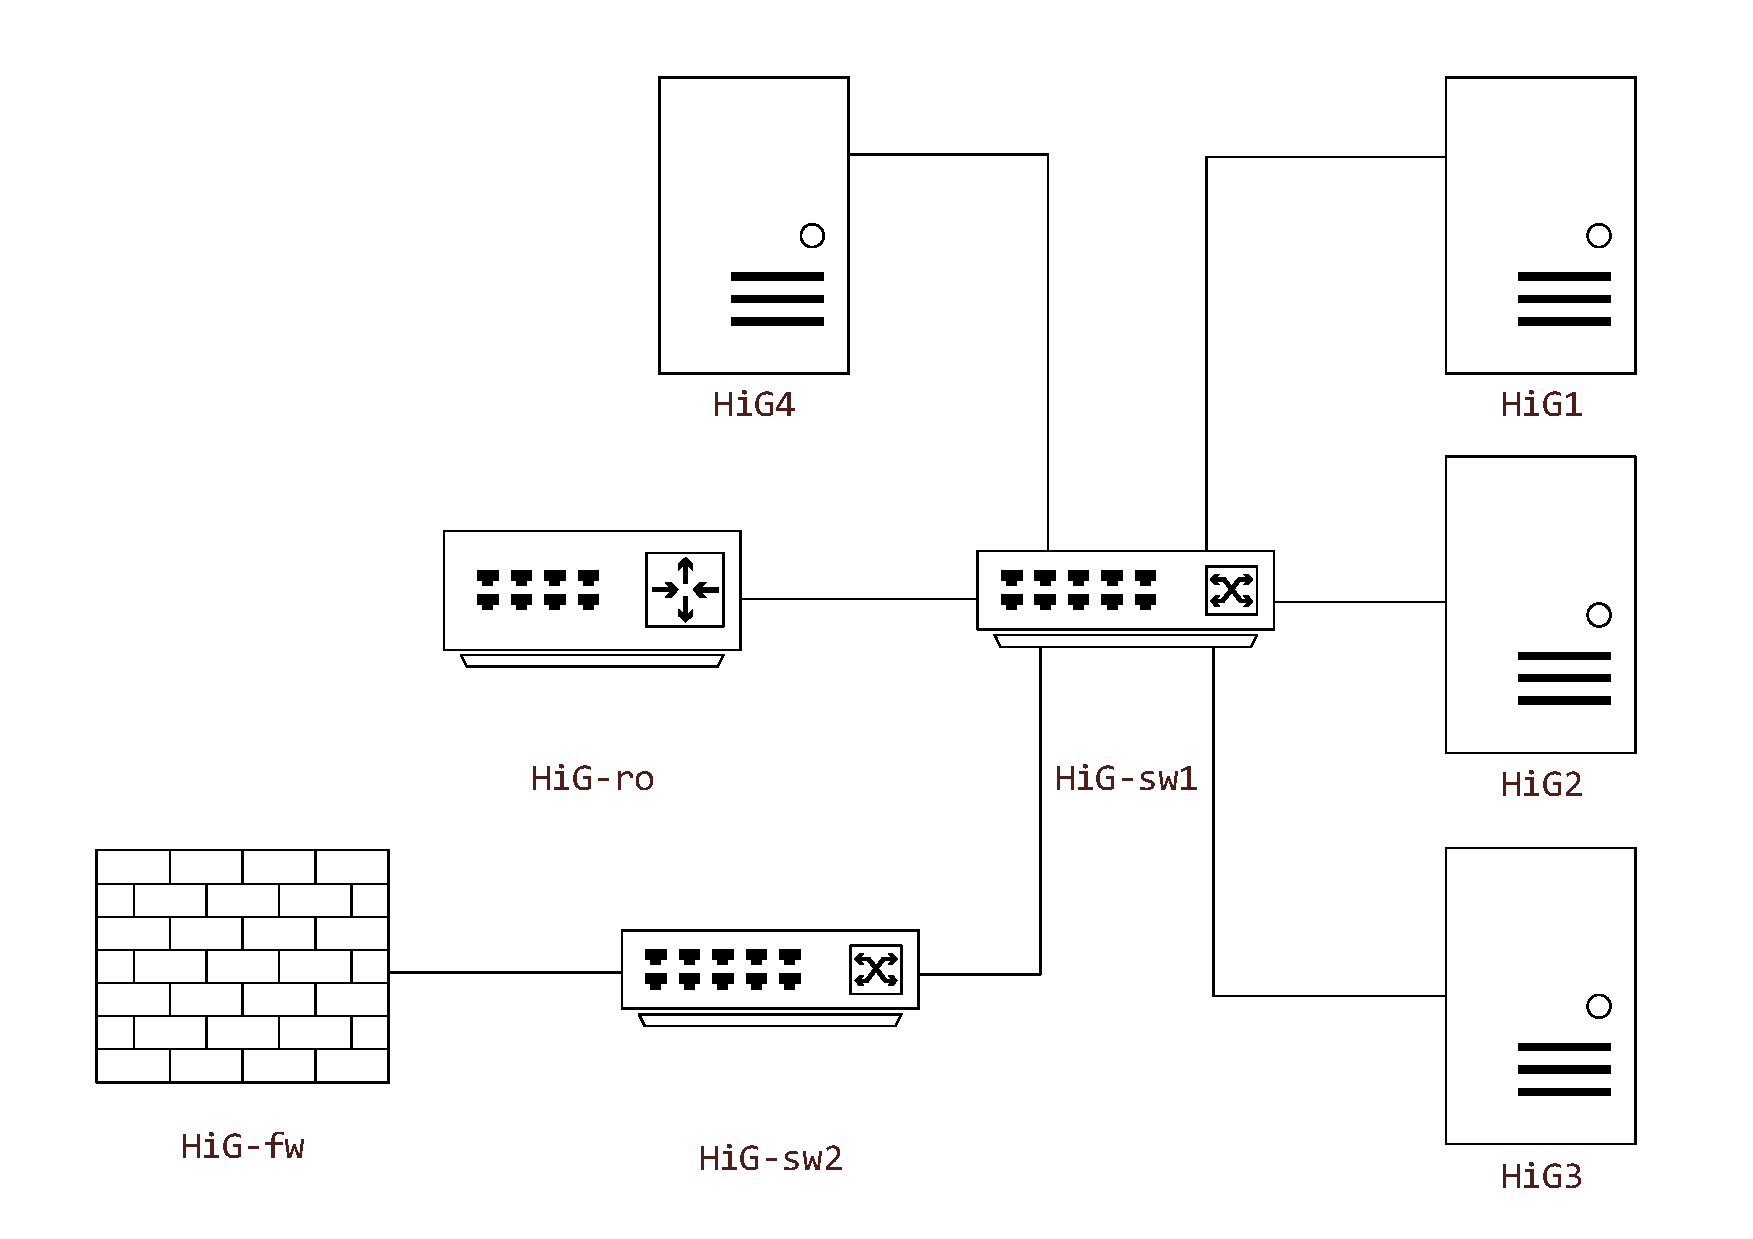
\includegraphics[scale=0.4]{img/labmiljo}
    \caption{Labmiljø}
    \label{laboppsett}
\end{figure}


\subsubsection{Produksjonsserveren}
Spesifikasjonene på bladeserveren:
\begin{itemize}
\item 4 CPU-er med 4 kjerner a x.x GHz
\item 32 GB RAM
\item Debian 6
\end{itemize}
Programvare:
\begin{itemize}
\item Debian 6
\item Apache2
\item MySQL
\item Icinga 1.8.4
\item SNMPtrapd
\item SNMPtt
\item Graphite
\item Metricinga 
\item sendmail
\end{itemize}
\subsubsection{Enhet for overvåkning av servermiljø}
For å overvåke temperatur og luftfuktighet på serverrommet ble det kjøpt inn en NetBotz 200 med støtte for opp til 12 eksterne sensorer \cite{netbotz},
som oppfyller kravene gitt i oppgavebeskrivelsen. 

\section{Produksjonsserver}
“Quis custodiet ipsos custodes?” er et latinsk uttrykk som kan oversettes med “hvem passer på de som passer på?”. I en overvåkningsløsning er det viktig å stille spørsmålet; hva skjer hvis overvåkningsserveren går ned? Et forslag under prosjektet var å legge overvåkingsserveren på et Xen/Vmware-cluster. Men dette ble etter noe omtanke stemplet som en dårlig ide. Dersom clusteret gikk ned ville også overvåkingsserveren gå ned. Det ble derfor bestemt at denne skulle være en egen fysisk boks. 

For å sikre tilgjengeligheten til Icinga ytterligere, er det også mulig å sette opp et redundant oppsett der alle Icinga-installasjoner kan dele resultater av sjekker mellom seg. Ekstra viktig vil et slikt oppsett være dersom man knytter overvåkningssystemet mot SLA-er. Dersom en mister data om oppetid og tilgjenglighet på en tjeneste, vil man ikke lenger kunne vise hva den har vært.

En annen utfordring var å vite hvor kraftig hardware serveren trengte. Her ble referanselisten til Icinga lagt til grunn \cite{icingainaction}, hvor mange organisasjoner har lagt inn informasjon om sine oppsett. Etter avtale med oppgragsgiver ble det bestemt å sette opp en bladeserver, som eventuelt kunne byttes med noe kraftigere dersom det skulle bli nødvendig. 

\subsection{Installasjon}
I pakkebrønnen for debian-stable fantes bare versjon 1.0.2 av Icinga, i backports lå 1.7.1. Icinga opprettholder en egen pakkebrønn - ``The Debian Monitoring Prosject'' \cite{debmon}. Fra denne kunne versjon 1.8.4 installeres. I samråd med teknisk kontakt ved IKT-avdelingen ble det bestemt å bruke versjon 1.8.4 fra debmon.

\subsection{Konfigurasjonsfiler}
Ved standard installasjon av Icinga er konfigurasjonen delt opp i objekttyper med flere objekter i hver fil:
\begin{itemize}
\item contacts\_icinga.cfg  
\item generic-host\_icinga.cfg     
\item hostgroups\_icinga.cfg  
\item localhost\_icinga.cfg  
\item timeperiods\_icinga.cfg
\item extinfo\_icinga.cfg   
\item generic-service\_icinga.cfg   
\item services\_icinga.cfg
\item commands.cfg
\end{itemize}
Dette var uoversiktelig og en oppdelt konfigurasjon var ønskelig, som også er anbefalt ved større installasjoner.. \cite{sysadmin} + nagios-boka. Det ble bestemt å sette opp følgdende hovedinndeling, med undermapper videre der det var hensiktsmessig:

\makeatletter
\newcount\dirtree@lvl
\newcount\dirtree@plvl
\newcount\dirtree@clvl
\def\dirtree@growth{%
  \ifnum\tikznumberofcurrentchild=1\relax
  \global\advance\dirtree@plvl by 1
  \expandafter\xdef\csname dirtree@p@\the\dirtree@plvl\endcsname{\the\dirtree@lvl}
  \fi
  \global\advance\dirtree@lvl by 1\relax
  \dirtree@clvl=\dirtree@lvl
  \advance\dirtree@clvl by -\csname dirtree@p@\the\dirtree@plvl\endcsname
  \pgf@xa=0.5cm\relax
  \pgf@ya=-0.5cm\relax
  \pgf@ya=\dirtree@clvl\pgf@ya
  \pgftransformshift{\pgfqpoint{\the\pgf@xa}{\the\pgf@ya}}%
  \ifnum\tikznumberofcurrentchild=\tikznumberofchildren
  \global\advance\dirtree@plvl by -1
  \fi
}

\tikzset{
  dirtree/.style={
    growth function=\dirtree@growth,
    every node/.style={anchor=north},
    every child node/.style={anchor=west},
    edge from parent path={(\tikzparentnode\tikzparentanchor) |- (\tikzchildnode\tikzchildanchor)}
  }
}
\makeatother
\begin{document}
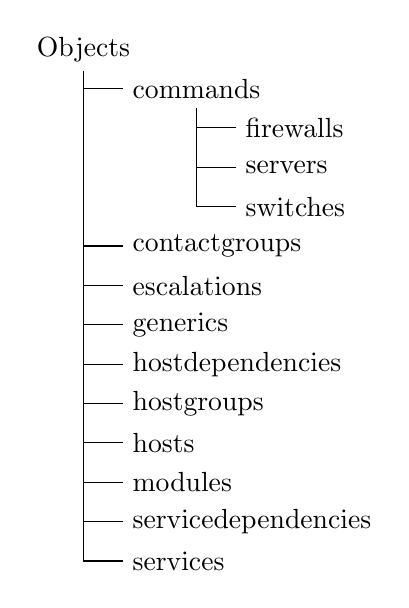
\begin{tikzpicture}[dirtree]
\node {Objects} 
    child { node {commands}
            child { node {firewalls} }
            child { node {servers} }
            child { node {switches} }
    }
    child { node {contactgroups} }
    child { node {escalations} }
    child { node {generics} }
    child { node {hostdependencies} }
    child { node {hostgroups} }
    child { node {hosts} }
    child { node {modules} }
    child { node {servicedependencies} }
    child { node {services} };
\end{tikzpicture}

Det ble testet ut et par verktøy for å administrere konfigurasjonsfilene NConf \cite{nconf} og NagiosQL \cite{nagiosql}. Disse ble valgt bort til fordel for manuel konfigurering da det ikke støttet oppdeling av konfigurasjon og kunne ikke kombineres med manuell konfigurasjon. I samråd med oppdragsgiver ble det avgjort av manuell konfigurasjon oppfyller kravet “Det skal være enkelt å legge til nye enheter for overvåking”.

\subsection{Bruk av hostgroup}
Som nevnt i /ref{der vi snakker om det} knyttes et service-objekt til et host-objekt og et command-objekt for at det skal kjøres en sjekk. For å slippe å skrive et service-objekt for hvert host-objekt benyttes gruppering av host-objekter i hostgroup. For å vise hvordan dette er satt opp vises et eksempel for hvordan dette er satt opp for MySQL-servere:

\begin{lstlisting}
define hostgroup {
        hostgroup_name mysql_servers
        alias MySQL Servers
}
\end{lstlisting}
Dette vil si at alle hosts som er medlem i hostgroupen vil få utført sjekkene som er definerert i servicen. For å legge til en host i denne gruppen kan hosten være definert på følgende måte.

\begin{lstlisting}
define host {
use		generic_windows_host
address	10.60.0.21
host_name	HiG2
alias		HiG2
hostgroups	debian_servers, mysql_servers
}
\end{lstlisting}
For å legge alle SQL serverne i en felles gruppe er det laget en egen SQL\_Servers host group. Dette gjøres for å gruppere alle SQL serverne uavhengig av hvilken database type som brukes. 

\begin{lstlisting}
define hostgroup {
hostgroup_name sql_servers
alias SQL Servers
hostgroup_members mysql_servers, mssql_servers, oracle_servers
}
\end{lstlisting}
Da kommandoene er definert lages servicen som som binder SQL serverens hostgroup og kommandoen.

\begin{lstlisting}
define service {
service_description MySQL Connection Time
use generic-service
name mysql_connection_time
hostgroup_name mysql-servers
check_command check_mysql_health!connection-time!0.1!0.4
}
\end{lstlisting}

Figur \ref{sql} viser en visuel fremstilling av hvordan alt dette henger sammen for alle SQL-servere:

\begin{changemargin}{-1cm}{-1cm}
\begin{figure}
    \centering
    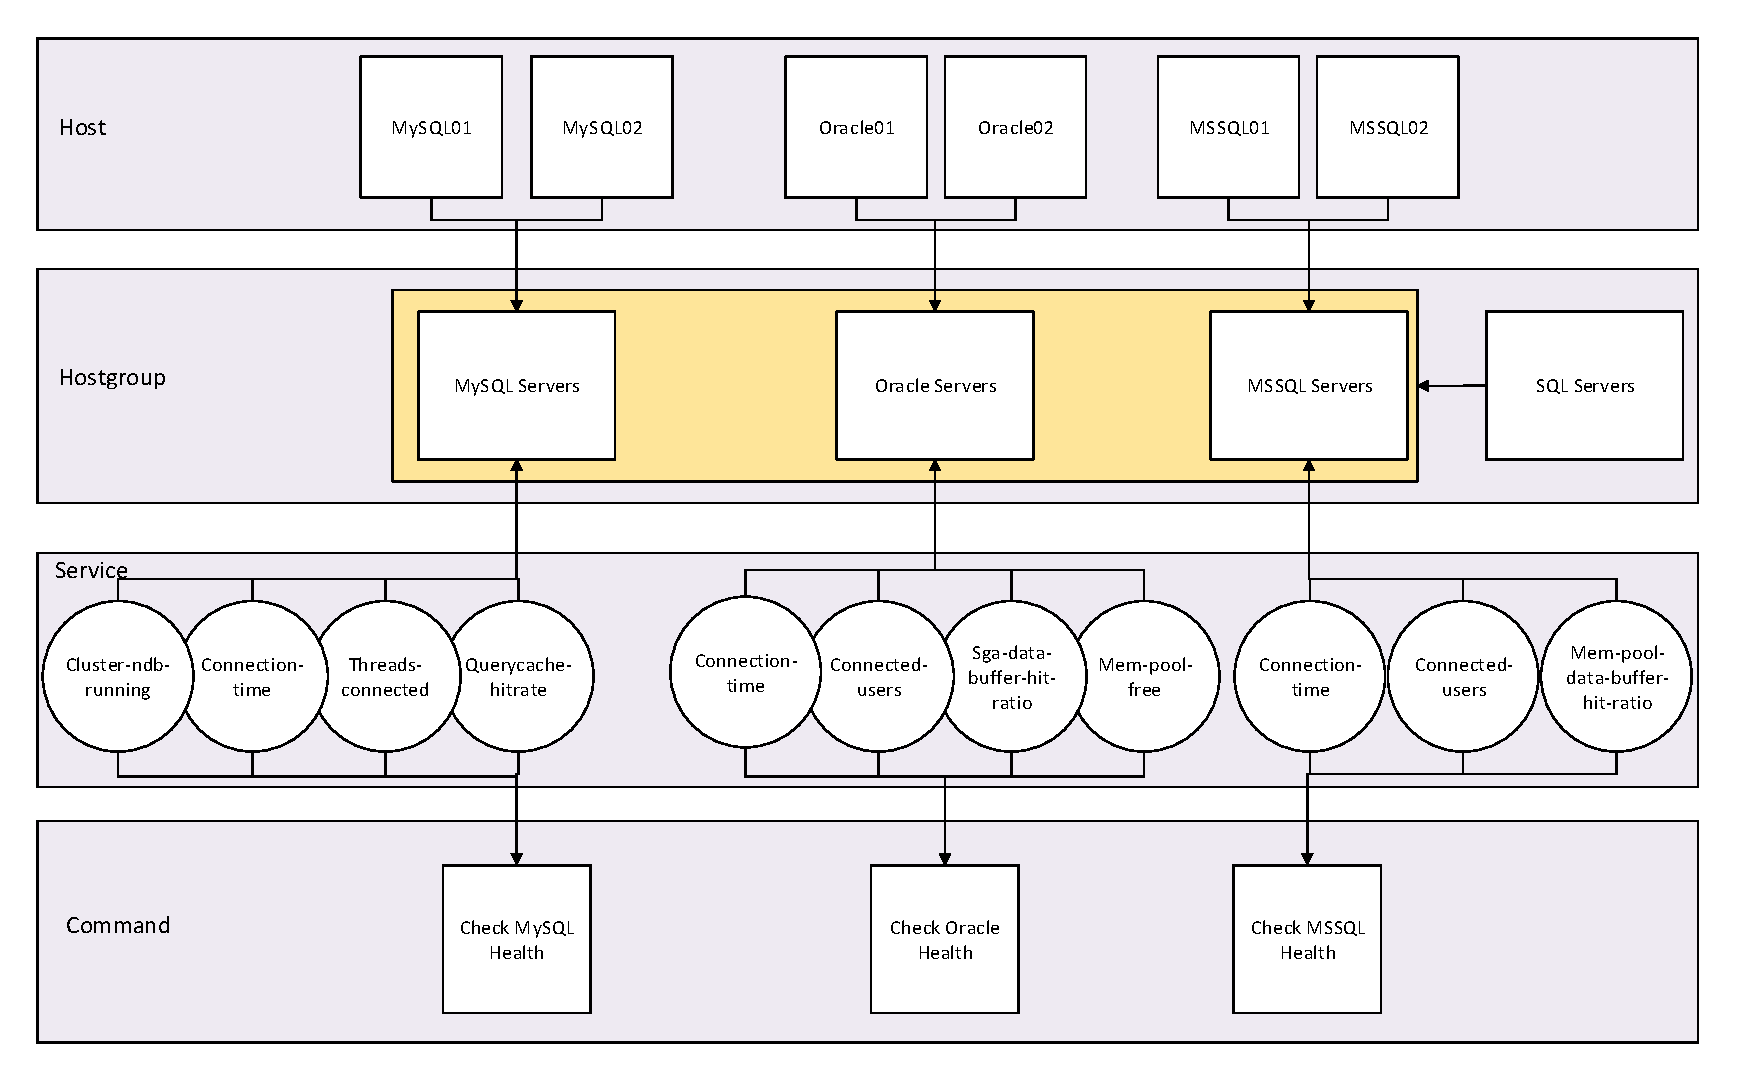
\includegraphics[scale=0.55]{img/sql}
    \caption{Visualerins av oppset for MySQL-server}
    \label{sql}
\end{figure}
\end{changemargin}
\clearpage


\section{Generering av grafer}
I utgangspunktet ble det bestemt at ytelsesdata skulle holdes utenfor oppgaven. Det ble likevel satt opp en løsning for å visualisere ytelsesdata fra sjekkene med programmet graphite. Dette ble gjort fordi det var ønskelig å kunne etablere en baseline for tjenestene slik at bedre grenseverdier kunne settes.

For å sette opp eksportering av ytelsesdataen benyttes et vanlig command-objekt i Icinga:

\begin{lstlisting}
define command {
command_name            rotate_perf_service
    command_line            /bin/mv /usr/local/icinga/var/perfdata/service-perfdata /usr/local/icinga/var/perfdata/logs/service-perfdata.$TIMET$
}
\end{lstlisting}
 Icinga.cfg må konfigureres til å benytte dette:

\begin{lstlisting}
process_performance_data=1
service_perfdata_file=/usr/local/icinga/var/perfdata/service-perfdata
service_perfdata_file_processing_command=rotate_perf_service
service_perfdata_file_template=[SERVICEPERFDATA]\tDATATYPE::SERVICEPERFDATA\tTIMET::$TIMET$\tHOSTNAME::$HOSTNAME$\tSERVICEDESC::$SERVICEDESC$\tSERVICEPERFDATA::$SERVICEPERFDATA$service_perfdata_file_processing_interval=200
\end{lstlisting}

For å transformere ytelsesdataene til riktig format for graphite benyttes metricinga \cite{metricinga}. Dette scriptet sjekker spool-mappen én gang i minuttet etter filer som enda ikke er prosessert og sender data inn til carbon (graphite). 
Gjennom graphite vil det dermed grafes basert på performance data på riktig format fra alle service-checks som kjører en command.

Det ble også testet å modifisere scriptet til å legge outputen til service-sjekkene direkte til en mysql-database, som vist i vedlegg /ref{metricinga diff}. Dette ble gjort for å oppfylle kravet fra oppgavebeskrivelsen om at alle henvendelser skal lagres i database. Men det viste seg at dette ville bli så mange rader at dette ble avgjort til ikke å være hensiktsmessig i samråd med oppdragsgiver. Som et alternativ til dette kan en ta inn all data til graphite, men aggrigere det etter en viss tid. Dataene kan da eksporteres fra graphite til videre bruk.

\section{Overvåkning av Windows-servere}
For overvåkning av Windows vil NSClient++ bli brukt. NSClient++ er et program som brukes for  å kommunisere med ulike agenter og over ulike protokoller på en ekstern server. I dette prosjektet brukes den for å hente ut informasjon via NRPE-agenten og å kjøre WMI-spørringer mot en Windows-server. NSClient har en konfig fil som genereres under installering. 

NSClient++ er valgt fordi klienten oppdateres hyppig \cite{nsclient}, og det er den agenten som blir referert i Icinga/Nagios dokumentasjon \cite{icingawin}. Med NSClient++ kommer også forhåndskonfigurerte plugin-er, for eksempel for å sjekke minne, CPU, og harddisk.

For installering av NRPE-agenten og mulighet for WMI-spørringer ble det laget en veiledning /cite{nsclientguide} som forklarer hva som skal installeres. Her er det laget en egen konfig fil som har kun funksjonaliteten vi trenger. 

\section{Overvåkning av Linux-servere}
Overvåkning av standard Linux-servere skjer utelukkende ved bruk av NRPE. 

For Debian-servere kan denne installers fra pakkebrønnen “stable” med kommandoen:

\begin{lstlisting}
apt-get install nagios-nrpe-server nagios-plugins-basic
\end{lstlisting}

For Red Hat og CentOS må det benyttes en tredjeparts “pakketing” som EPEL eller DAG før nrpe-server kan installeres med yum.

Konfigurasjonen er lik som ved Windows. Det følger ikke med noen plugin-er når en installerer nagios-nrpe-server, derfor installeres også pakken “nagios-plugins-basic”.

\section{Utrulling av agenter}
NSclient++ kan lastes ned som en MSI-pakke, som kan pushes til servere med en GPO. Konfigurasjonsfilen må enten legges inn i MSI-pakken eller pushes over GPO for seg selv. Grunnen til dett ikke er benyttet er at IKT-avdelingen ønsket å gjøre installasjonen manuelt for å ha mest mulig kontroll og gjøre utrulling i faser, for å sikre at installasjonen ikke medførte uforutsette probemer. Det ble laget en veiledning på hvordan denne klienten skal installeres, og hvilke opsjoner som er relevant. Denne finnes i vedlegg \ref{nsclient++}.

For Linux servere installeres pakkene via pakkebehandleren, som nevnt i xx. IKT-avdelingen har for tiden ikke så mange Linux-servere, så noen automatisk utrulling vil ikke være så besparende. Dersom dette skulle være ønskelig kan et enkelt script som kobler seg til og kjører kommandoen for installering skrives. Konfigurasjonsfilen kan pushes over SCP.

For annen infrastruktur brukes for det meste SNMP for å hente ut informasjon. Dette konfigureres på hver enkelt enhet, og krever vanligvis ikke noe ekstra programvare installert. I noen spesielle tilfeller brukes egne API-er for å hente ut informasjon, som for eksempel for VMware. Her må Icinga serveren ha tilgang til å bruke API-et, som vanligvis konfigureres på hosten.

\section{Lokale ressurser}
For både Linux- og Windows-servere er det satt opp noen grunnsjekker som skal kjøres på alle servere. Dette er CPU-last, harddiskplass og minnebruk. Hver sjekk er definert i et service-objekt der hostgroup-ene er satt til “windows\_servers” og “linux\_servers”. 

For alle disse sjekkene er det mulig å anngi grenseverdier både som prosentandel og absolutte tall og sjekke mot både andel ledig eller andel brukt. 
\subsection{Disk}
Lav diskplass kan skape problemer for applikasjoner som lagrer data, logging kan stoppe, og ved høyt minneforbruk og bruk av virtuelt minne vil ikke diskplass kunne utnyttes og applikasjoner kan stoppe å fungere.

Linux:

For å sjekke ledig plass på harddisken benyttes Nagios-sjekken “Check\_disk”. 
Check\_Disk
\begin{lstlisting}
./check_disk -w 8% -c 4% -e
\end{lstlisting}
Svar: 
\begin{lstlisting}
DISK OK| /=1232MB;15430;17359;0;19288 /lib/init/rw=0MB;402;452;0;503 /dev=0MB;394;443;0;493 /dev/shm=0MB;402;452;0;503
\end{lstlisting}
I sjekken over brukes oppsjoner slik at det gir en advarsel om det er 8 \% ledig diskplass, og vil gi kritisk varsel dersom det er 4 \% ledig diskplass.

For windows servere med mange disker brukes oppsjonen -CHECKALL som gir en oversikt over alle diskene på serveren. Her brukes samme opsjoner for advarsler og kristiske varsler.

-CheckDisk fra nsclient++

\subsection{CPU}

Overvåkning av CPU vil kunne hjelpe til med å indikere problem som ressursproblemer, flere CPU-krevende applikasjoner på samme server eller at en applikasjon bruker all CPU-kraft.  

På Windows-servere benyttes “CheckCPU” fra NSClient++ for å sjekke CPU-last. Her legges det ved tre opsjoner i sjekken som spesifiserer tidsintervallet for datagrunnlaget, grensen for når det skal gis en advarsel og når det skal vises som en kritisk feil.

Check\_CPU
\begin{lstlisting}
./check_nrpe -u -H 10.60.0.22 -p 5666 -c CheckCPU -a time=5m warn=80 crit=90
\end{lstlisting}
I Figur \ref{cpustrain} returnerer CPU-sjekken “OK”. Dette er hentet fra gjennomsnittsbruk av CPU over 5 minutter. Like under ser vi at testen er kritisk på grunn av et gjennomsnittsbruk av CPU på 96 \%. I Figur \ref{CPUSTRAIN} ser vi at alle de fire CPU-kjernene jobber oppmot maksimalt. Et batch-script ble kjørt lokalt på serveren som ble overvåket for å generere CPU-bruk.
\begin{lstlisting}
## winloop.bat
##
# Kjører loop.bat 10 ganger.
#
@echo off
for /l %%x in (1, 1, 10) do (
    start loop.bat
)

# loop.bat
@echo off
:loop
GOTO loop
\end{lstlisting}

\begin{figure}
    \centering
    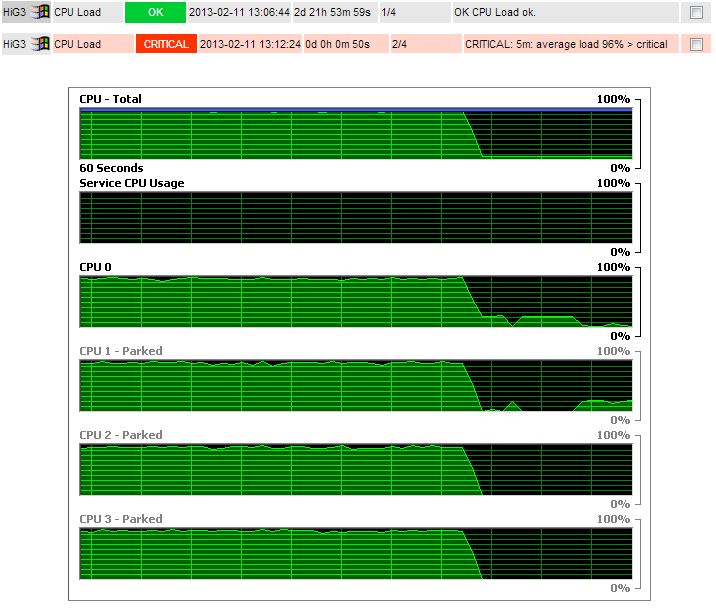
\includegraphics[scale=0.6]{img/cpu_test_hig3}
    \caption{CPU-bruk for HiG3}
    \label{cpustrain}
\end{figure}


For Linux baserer sjekk av CPU-bruk seg på “load” \cite{loadavg} \cite{wiki:loadavg}. Dette er i hovedsak et gjennomsnitt for hvor mange prosesser som bruker eller venter på CPU, men disk- eller nettverks I/O kan også spille inn. For maskiner med flere kjerner og/eller CPU-er vil dette fortone seg annerledes da en kan utføre flere prosesser parallellt. Load-tallene må deles på antallet CPU-kjerner for at det skal kunne brukes samme grenseverdier uavhengig av hvor mange kjerner serveren har. Dette gjøres med opsjonen “r”.

Tallene som hentes ut er gjennomsnittet for de siste 1, 5 og 15 minuttene. Det er mer interessant hvis load-en er høy over lengre tid, derfor er grenseverdiene lavere for 5 og 15 minutters intervallene.

check\_load fra nagios-plugins:
\begin{lstlisting}
load average: 0.65 0.42 0.36

check_command                   check_nrpe!check_dist_load!0.9,0.7,0.5 1.2,1.0,0.9

command[check_dist_load]=/usr/lib/nagios/plugins/check_load -r -w $ARG1$ -c $ARG2$
\end{lstlisting}

\subsection{Minne}
Datamaskiner som bruker opp tilgjengelig minne må skrive til disk for å få plass til mellomlagrede data. Data som må hentes fra disk vil ha en betydelig høyere aksesstid enn når fysisk minne brukes til mellomlagring \cite{wiki:mem}. 
Kontinuerlig høyt minneforbruk kan være en indikasjon på flere minnekrevende applikasjoner på samme server, en applikasjon har minnelekkasje, eller at mengden minne ikke strekker til.

Hva en prosess kan kreve. Virtuelt minne teknologi. CheckMem fra NSClient++

\begin{lstlisting}
Check_Memory
./check_nrpe -u -H 10.60.0.22 -p 5666 -c CheckMem -a MaxWarnUsed=80% MaxCritUsed=90% type=physical

Svar
OK memory within bounds.|'physical memory %'=16%;80;90 'physical memory'=1G;4;5;0;6
\end{lstlisting}

Opsjoner sendes med som gjør at sjekken gir warning når mer enn 80 \% av fysisk minne er brukt, når minneforbruket overstiger 90 \% blir minneforbruket kritisk.

For Linux benyttes plugin check\_mem \cite{checklinuxmem}

\section{Tjenester}
IKT-avdelingen ønsket å overvåke tjenester og prosesser på serverne. Prossesser er instanser av programmer som kjører. Tjenester er prosesser som kjører i bakgrunnen. 

Overvåkning av tjenester vil innebære å se på om én eller flere prosesser kjører
til en hver tid. NSclient++ har muligheten til å se om en bestemt prosess eller tjeneste kjører eller har stoppet. Her spesifiserers det hva prosessen eller tjenesten heter og sjekken svarer på om denne finnes i prosesstabellen.
\begin{lstlisting}
define service {
        service_description     DHCP Service
        hostgroup_name          dhcp_servers
        check_command           check_nrpe!CheckServiceState!DHCPServer=started ShowAll
        use                     generic_service
}

define service {
  use            generic_service
  hostgroup_name       linux_servers
  service_description     NRPE Check my process
  check_command        check_nrpe!check_process!sshd 1:40
}
\end{lstlisting}
linux-plugin fra nagios-plugins: check\_procs 

Å se at en tjeneste kjører via Windows kan gi falsk informasjon. Et eksempel her er Microsoft's terminal services. Tjenesten står som kjørende i Windows, men brukere får ikke koblet til. Dette kommer av at tjenesten har hengt seg, uten at den står som “stoppet”. Dette merkes ikke før brukere ringer inn og beskriver problemet \cite{serviceproblem}. Som nevnt i x.x vil en bedre sjekk være å teste selve tjenesten, som i neste delkapittel.

\subsection{LDAP, DNS og DHCP}

Tjenester som LDAP-autentisering, DNS-oppslag og DHCP-leasing er en viktig del av tjenestene IKT-avdelingen leverer.

LDAP-tjenesten gjør at brukere får logget på trådløse nettverk og autentisert seg for andre tjenester IKT-avdelingen leverer \cite{ldap}.

DNS oppslag gjøres hver gang en enhet skal oversette en IP-adresse til et hostname eller omvendt. Uten DNS vil ikke enheten kunne kontakte andre enheter ved å benytte hostname, som brukes i f.eks web-adresser \cite{dns}. 

Når en ny enhet kobles til nettverket vil denne få tildelt en IP-adresse av DHCP-serveren. Samtidig får den informasjon om gateway og DNS-servere. Uten dette vil ikke enheten få kommunisert med andre enheter på nettverket \cite{dhcp}.

Sjekkene for alle de tre tjenestene vil bli gjort direkte fra Icinga-serveren. Denne står i et eget nettverk. Derfor vil det kunne oppstå situasjoner der Icinga rapporterer at tjenestene fungerer, men det ikke fungerer for brukere tilkoblet andre nettverk. En løsning på dette kan være å kjøre sjekkene via en server i hvert nettverk brukere er tilkoblet.


\subsubsection*{LDAP}

For å overvåke LDAP-tjenestene benyttes pluginen “check\_ldap” som følger med i pakken nagios-plugins-basic. Pluginen kobler til LDAP-tjenesten og prøver å autentisere en bruker. Her vil sjekken returnere OK, om den fikk autentisert. 

Performancedata har blitt samlet inn for å sette grenseverdier for når Icinga skal gi varsel om treg innlogging. I Figur \ref{ldapauth-inv} ser vi at tjenesten sjekket på fire LDAP-servere, over en måneds periode bruker rundt 0.0044 sekunder på å autentisere. Ut ifra dataen som er samlet settes warning settes til 0.01 sekund, og kritisk settes til 0.02 sekunder.

\begin{figure}
    \centering
    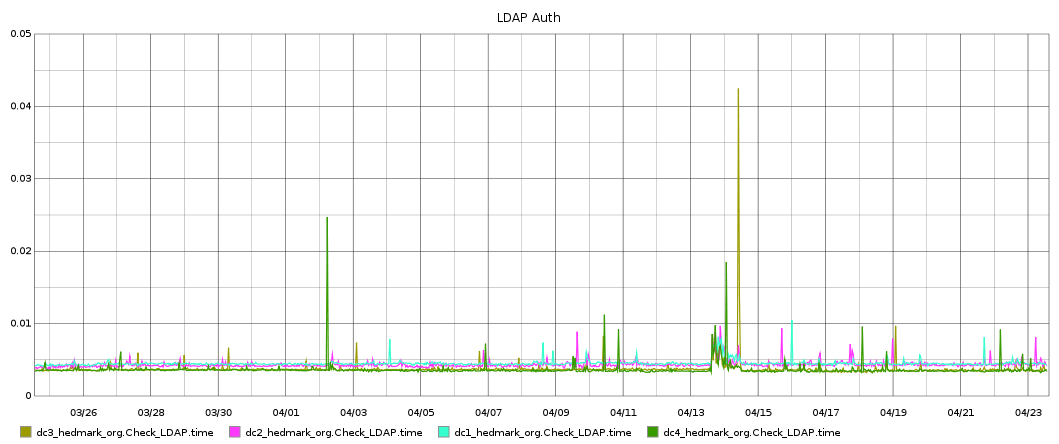
\includegraphics[width=1.0\textwidth]{img/ldap-auth-inv}
    \caption{Data fra Graphite (sekund)}
    \label{ldapauth-inv}
\end{figure}


\subsubsection*{DNS}

DNS overvåkes av pluginen “check\_dns”. Denne på samme måte som “check\_ldap” kobler til selve tjenesten. Denne fungerer ved å gjøre et DNS-oppslag på en spesifikk IP-adresse, og verifisere dette mot et satt hostname. Dersom dette stemmer vil plugin-en returnere OK, sammen med ytelses-data på hvor lang tid oppslaget tok.

Figur \ref{dns-inv} viser data samlet inn fra to DNS servere over 30 dager. Disse dataene viser forventet tid for et oppslag, og utifra dette ble grenseverdien for WARNING satt til 0.01 sek og CRITICAL til 0.02 sek.

\begin{figure}
    \centering
    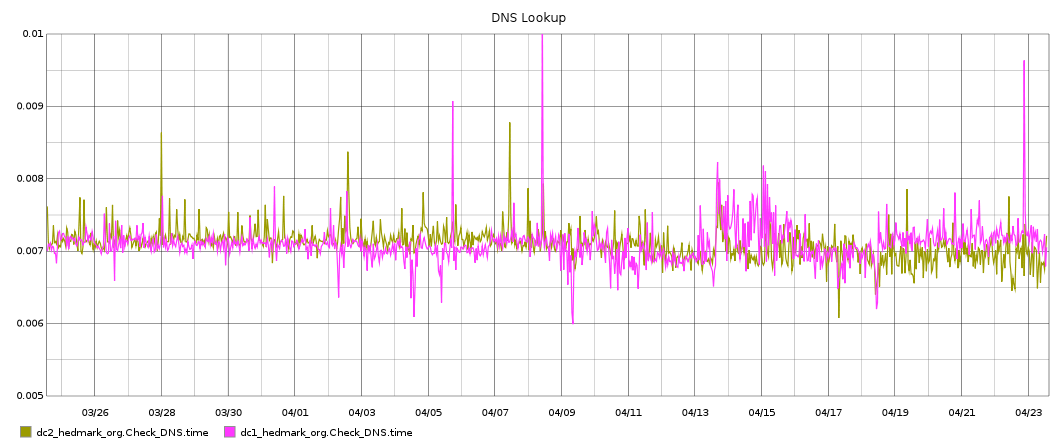
\includegraphics[width=1.0\textwidth]{img/dns-inv}
    \caption{Data fra Graphite (sekund)}
    \label{dns-inv}
\end{figure}


\subsubsection*{DHCP}

DHCP tjenesten overvåkes med pluginen “check\_dhcp”. Denne sender en DHCPDISCOVER-pakke til DHCP-serveren. Hvis DHCP-tjenesten fungerer får pluginen en DHCPOFFER-pakke som respons. Dersom denne inneholder en korrekt lease, returnerer pluginen OK til Icinga sammen med tiden det tok.

\subsubsection{Counters}
Mange interne applikasjoner brukes via Terminalservere, her er det viktig å kunne levere et stabilt system til brukerne, ofte kan terminalservere belastes mer i perioder, det blir da naturlig å overvåke hvor mange som bruker disse serverne, for å kunne sette inn nye servere, og se hvem som blir belastet mest.

Ved å bruke NRPE sjekkes windows performance counters direkte. I Figur \ref{ts-skole-usage} checkterminalservices er bruken for en uke samlet inn og kan brukes videre til å evalure terminalserver lasten.

Kommando som er brukt for å samle denne datoen er følgende:

\begin{figure}
	\centering
	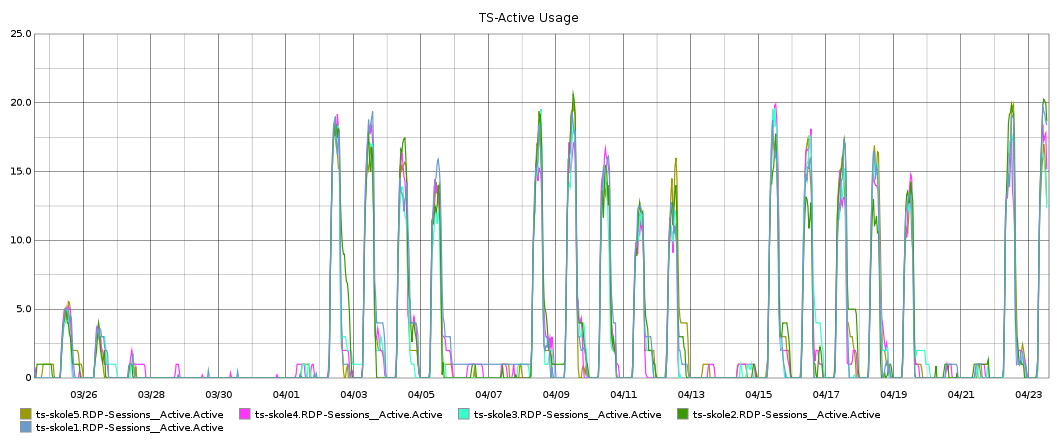
\includegraphics[width=1.0\textwidth]{img/ts-skole-usage-inv}
	\caption{Data fra Graphite (Terminal service aktive brukere)}
	\label{ts-skole-usage}
\end{figure}



\subsection{Sjekk av redundante oppsett}
En ordinær plugin henter status for en service som kjører på én host. Ved redundante oppsett vil det ikke nødvendigvis være kritisk om en av nodene er nede. For å vurdere statusen av et cluster kan en kjøre en sjekk på hver enkelt host som kjører den gitte servicen, få tilbake resultat fra hver, og ta en vurdering basert på disse resultatene samlet.

For å overvåke redundante oppsett, har pluginene check\_multi og check\_cluster blitt vurdert.  Forskjellene mellom disse er at check\_cluster i motsetning til check\_multi parser den lokale status.dat filen og ser hvilken tilstand en service eller en host er ved siste sjekk. Pluginen check\_multi derimot kjører aktive sjekker mot spesifiserte hosts, og en kan definere comparison operator som vil bli sjekket mot de returnerte resultatene.

Med check\_multi kan en benytte en eller flere egendefinerte kommandoer som parametere. Disse vil bli parses av check\_multi og kan inneholde alt i fra “echo Hello” til mer avanserte perl script, som kjøres ved hjelp av eval. For å evaluere resultatene kan en definere kriterier som gir et varsel (her brukes standard Icinga-tilstander). 

Eksempel:
\begin{lstlisting}
command [ HTTP_Node1 ] = check_http -H 192.168.2.10
command [ HTTP_Node2 ] = check_http -H 192.168.2.11
command [ HTTP_Node3 ] = check_http -H 192.168.2.12
state [ WARNING ] = COUNT(WARNING) > 2
state [ CRITICAL ] = COUNT(CRITICAL) > 3
\end{lstlisting}
For check\_cluster spesiferes det om det er et host- eller service-cluster en skal sjekke. Deretter spesifiseres parametere med navn på host og service, og hvor mange hosts eller services som må være nede før at det skal varsles med warning eller critical. Siden check\_cluster kjører lokalt på Icinga-serveren vil den ikke bruke noe nettverkstrafikk, noe som er positivt. Ulempen er at den ikke gir noen informasjon om hvilken host som er nede eller hvilken host en service feilet på. Det vil si at den gir bare en overordnet status for det redundante oppsettet     

Under vises et eksempel hvor servicen Check HTTP for host-objektene localhost, HiG2, HiG3, og HiG4 blir kjørt og vil gi WARNING om 1 er nede og CRITICAL om 2 er nede: 
\begin{lstlisting}
check_cluster --service -l "Check HTTP"  -d $SERVICESTATEID:localhost:Check HTTP$, $SERVICESTATEID:HiG2:Check HTTP$ ,$SERVICESTATEID:HiG4:Check HTTP$  -w @1 -c @2
\end{lstlisting}

\subsection{Microsoft Exchange}

Exchange er en kritisk tjeneste for fylkeskommunen. Her routes og lagres all e-post som sendes ut og inn av alle brukere. 

Gjennom perfmon har en tilgang til en rekke viktige tall \cite{exchange} for å måle ytelsen i Exchange. Disse kan overvåkes over NRPE med check\_counter i NSClient++.
\begin{itemize}
	\item Antall tilkoblinger
	\item Gjennomsnittlig responstid
	\item Antall meldinger sendt per sekund. Ved høye tall kan det være mistanke om at mail-serveren blir brukt til spam, eller at det er zombier på nettverket.
	\item Antall LDAP-søk som gir timeout. Feil mot AD.
	\item Økning i SMTP-køen
\end{itemize}

Microsoft har gitt ut egne anbefalinger til grenseverdier \cite{exchangethresholds}.

I tillegg til disse var det ønskelig med en sjekk som testet hele e-post-oppsettet. Til dette benyttes pluginen “check\_email\_delivery” \cite{exchange}. Her sjekkes det at en e-post kan sendes fra SMTP-serveren. E-posten som sendes ut inneholder en unik ID. Videre kobler pluginen seg til IMAP-tjenesten og sjekker om e-posten med den unike ID-en kom frem. Antall sekunder for hele round-tripen blir målt. Helst skulle en her koblet til en SMTP-server som står utenfor nettverket, men dette var det ikke andledning til.

Det sjekkes også at websiden for Outlook Web Access er tilgjengelig gjennom pluginen “check\_http”. Her burde en nok også sjekket om det var mulig å logge inn.

\section{Databaser}
Tre forskjellige databasemotorer benyttes av IKT-avdelingen. Disse er MySQL, MSSQL og Oracle DB. Disse har ulik arkitektur og virkemåte \cite{databasecomparison}, og derfor blir ikke de samme parameterene overvåket på alle. Felles for alle er:

Connection time (tid det tar å koble til SQL serveren).
Connected users (antall aktive sessioner mot SQL serveren).
Cache hit rate (antall spørringer som blir hentet fra cache i et tidsinterval).

Disse er valgt

Spesifikke
\begin{itemize}
\item MySQL: Slow queries (antall trege spørringer SQL serveren utfører i et tidsinterval).
\item MSSQL: Lazy writes
\item Oracle: Free table space (Plass ledig for tabellene).
\item Oracle: Switch interval (Overvåker load).
\end{itemize}

\subsection*{Connection time}
Connection time gir beskjed dersom det ikke er mulig å koble til SQL serveren. Hvis denne sjekken gir en timeout, er det fordi sjekken ikke får kontakt på porten til SQL tjenesten. Her definerers det parametere for hvor lang tid det burde ta å koble til. Hvis tilkoblingstiden blir for lang varsler Icinga om dette. Grenseverdier her er valgt ut fra gjennomsnittlig tid det har tatt å koble til i perioden denne har vært operativ. Data for tilkoblingstiden har blitt samplet over 30 dager.

\subsection*{Connected users}
Connected users sjekker hvor mange sessioner som er koblet til database tjenesten (per instanse for Oracle DB). Antall aktive sessioner blir samlet inn om hver enkelt database. Derfor defineres thresholds ut fra hvor mange brukere som er koblet til over en periode. Da plukkes uvanlige bruksmøstre opp og kan videre studeres.

\subsection*{Cache hit}
Cache hit er hvor ofte data hentes ut fra databasemotorens egen cache, slik at dataen ikke leses fra disk, Dette sparer diskene for I/O operasjoner. Hvis cache hit ligger på et høyt nivå (90-100 \%), indikerer dette at tabellene det spørringes mest mot lagres i cache. Når cache hit ligger under 90 \% kan dette være et resultat av at serveren ikke har nok minne til å lagre tabellene i cache. Dette kan indikere et minneproblem.

Cache hiten er anbefalt fra Oracle sin side å ligge over 90 \% \cite{oraclecachehit}. 
For MSSQL er så nærme 100 \% cache hit et godt utgangspunkt. Dette indikerer at MSSQL klarer å lagre de mest brukte tabellene i minne. \cite{sqlmonitoring}
MySQL databasene til IKT-avdelingen lagrer all database data i minnet, så her vil det ikke være relevant å sjekke cache hit. Sjekken er satt opp slik at ordinære MySQL-servere vil kunne settes opp med denne sjekken i etterkant.

\subsection{Plugin} %???
For at Icinga-serveren skal kunne snakke med de forskjellige database-motorene trengs en klient for hver av de. 

\subsubsection{Oracle}
Databaseklienten finnes på Oracle sine nettsider \cite{oracleclient}. Den finnes ikke som en deb-pakke, som som brukes for Debian. Det finnes derimot en rpm-pakke, som brukes av blant annet Red Hat. Alien /cite\cite{debian:alien} ble brukt til å konvertere rpm-pakken over til deb-pakke før installasjon på Icinga-serveren. 
\begin{lstlisting}
alien oracle-instantclient11.2-basic-11.2.0.3.0-1.x86_64.rpm 
dpkg -i oracle-instantclient11.2-basic-11.2.0.3.0-1.x86_64.deb
\end{lstlisting}
Videre trengs også en databasedriver, som gjør det mulig for Perl å benytte klienten. For oracle databaser brukes perl DBI driver for Oracle “libdbd-oracle-perl”.

På en Oracle server vil hver database ha sin egen instans /cite{http://searchoracle.techtarget.com/answer/What-s-an-Oracle-instance}. Det vil si at parametre som overvåkes vil være forskjellig fra database til database. Navnene til instansene legges derfor inn som en egendefinert variabel i hver enkel Oracle-servers host-objekt. Når pluginen kjøres sjekkes filen tnsnames.ora /ref{tnsnames} som inneholder tilkoblingsinformasjon for hver enkelt instans.
\begin{lstlisting}
ORA11 =
 (DESCRIPTION = 
   (ADDRESS_LIST =
     (ADDRESS = (PROTOCOL = TCP)(HOST = 127.0.0.1)(PORT = 1521))
   )
 (CONNECT_DATA =
   (SERVICE_NAME = ORA11)
 )
)
\end{lstlisting}
Check\_multi brukes så for å samle en Oracle servers instanser under samme service. Eksempelvis når cache hit sjekken kjøres, vil check\_multi utføre sjekken for alle instansene. Deretter vil svarene fra instansene samles under samme check cache hit sjekk i Icinga. Dette gjør det mer oversiktlig å overvåke oracle servere.

\begin{lstlisting}
define service {
...
check_command check_multi!check_oracle! -s dbinstances=$_HOSTDBINSTANCES$ -s host=$HOSTADDRESS$ -s mode=sga-data-buffer-hit-ratio -s warning=93: -s critical=90: -s user=$USER5$ -s pass=$USER4$
}

define command {
...
command_line	check_multi -r 32 -f /etc/icinga/objects/commands/check_multi/$ARG1$.cmd $ARG2$
}


eeval [ oracle_health ] =
    	my $chain = "";
    	foreach my $instance (split(/,/,'$dbinstances$')) {
            	$chain .= "-x \"command[ $instance ] = check_oracle_health --connect '$user$'\/'$pass$'\@'$instance' --mode '$mode$' --warning $warning$ --critical $critical$ \" ";
    	}
    	parse_lines("command [ check_oracle ] = check_multi -r 4 $chain");

\end{lstlisting}

\subsubsection{MySQL}
For MySQL ligger de nødvendige pakkene i Debians pakkebrønnen og kan installeres med apt. De nødvendige pakkene er “mysql-client”, for database koblingen og “libclass-dbi-mysql-perl”, som er en Perl-modul for å kunne koble til en MySQL-server. 
MSSQL
For MSSQL var det vanskelig å finne en databaseklient som er opensource. Her endte vi opp med FreeTDS \cite{freetds}, sammen med Perl-modulen “libdbd-sybase-perl”

Plugin
Plugin-ene som blir benyttet for databaser er skrevet av firmaet “Consulting \& Solutions” og heter “Check\_MySQL\_Health”, “Check\_Oracle\_Health” og “Check\_MSSQL\_Health” \cite{consol}

Disse må kompileres fra kildekoden. For å gjøre dette må en først konfigurere de med riktige parametere. Dette er de samme for alle tre plugin-ene.

\begin{lstlisting}
./configure --prefix=/usr/lib/nagios/plugins/ --with-nagios-user=nagios --with-nagios-group=nagios --with-perl=/usr/bin/perl --with-statefiles-dir=/tmp
\end{lstlisting}

Pluginen kompileres og legges i riktig bane ved å kjøre kommandoene

make
make INSTALL

For å koble til databaseserverne trengs servicebrukere i hver av de. Her holder det med minimale tilganger slik at denne ikke har tilgang til å endre tabeller og spørre etter info. Brukeren vil kun ha tilgang til å kjøre “Server administrasjon” kommandoer \cite{mysqlpriv}.

I MySQL brukes følgende kode for å opprette denne brukeren:
\begin{lstlisting}[language=SQL]
GRANT USAGE ON *.* TO 'icinga'@'10.60.0.20' IDENTIFIED BY 'Bachel0r'; 
\end{lstlisting}

Script for å opprette brukere i Oracle og MSSQL finnes i vedlegg /ref{sqlscript}.

Konfigurasjonen
Kommandoen konfigureres med muligheten for å bestemme hvilken sjekk som skal kjøre i \$ARG1\$.

Her brukes MySQL som eksempel men dette vil være lik på de andre forskjellige SQL serverne. 
\begin{lstlisting}
command_line $USER1$/check_truedatabase-motor>_health --hostname=$HOSTADDRESS$ --username=$USER5$ --password=$USER4$ --mode $ARG1$ --warning $ARG2$ --critical $ARG3$
\end{lstlisting}
\subsubsection{MySQL Cluster}

MySQL Cluster er et distribuert oppsett for MySQL. Ved IKT-avdelingen benyttes et MySQL Cluster med NDB som lagringsmotor, der databasene kjører i minnet. Et MySQL Cluster består av tre forskjellige nodetyper:

\begin{itemize}
	\item Management - her konfigureres clusteret og en setter opp hvor mange Data- og SQL-noder som kan kobles til.
	\item Data - oppbevarer dataene i RAM. Disse håndterer lastbalasering, replikering, failover og gjenoppbygging automatisk i mellom hverandre.
	\item SQL - MySQL servere som kobler seg til data-nodene for å hente og lagre data.
\end{itemize}

Den enkleste måten å hente ut statistikk om et MySQL Cluster er å benytte seg av mangement programmet “ndb\_adm” som kan hentes ut fra installasjonspakken til mysql-cluster \cite{ndbdownload}. I ndb\_adm kan en se hvor mange noder av hver type som er tilkoblet og minneforbruket til hver av datanodene. De plugin-ene som benyttes baserer seg på output fra “ndb\_adm”.

Antallet noder tilkoblet overvåkes med pluginen check\_ndbd \cite{ndbnode}. Her ble det gjort en endring i koden slik at serveren som ndb\_adm kobler seg til kan spesifiseres som en parameter.

For minnebruk ble det skrevet en egen plugin, da ingen eksisterende plugin ble funnet som tillot å spesifisere hvilke noder som skulle sjekkes. ID-ene til nodene som skal sjekkes ble satt opp som en egendefinert variabel i host-konfigurasjonen. Denne sendes til pluginen via service- og kommando-objektene, som vist under.

\begin{lstlisting}
define host {
	...
	_NODEIDS 2,3  ;Data-nodes IDs to check memory usage
}

define command {
	...
	command_line   $USER1$/libexec/check_ndb_mem.pl --host $HOSTADDRESS$ --nodes $ARG1$ --warning $ARG2$ --critical $ARG3$
}
\end{lstlisting}
\section{Applikasjoner}
Muligheten for å se om en applikasjon fungerer slik den skal er en viktig del av overvåkningen. Det er applikasjonene brukerne benytter seg av og vil sende inn feilmeldinger om. En applikasjons tilstand vil bestemmes av flere tjenesters status. I Icinga benyttes et servicegroup-objekt for å gruppere flere service-objekter.

Et praktisk eksempel på dette vises i Figur \ref{servicegroup_layout}. Her vil applikasjonen “Web App for ERP” være avhengig av webserveren for å vise web-grensesnittet til brukerne, en filserver for lesing og lagring av filer, en e-post-server for å sende og motta mail og en databaseserver som inneholder brukerinfo og andre tabeller. 

\begin{figure}
    \centering
    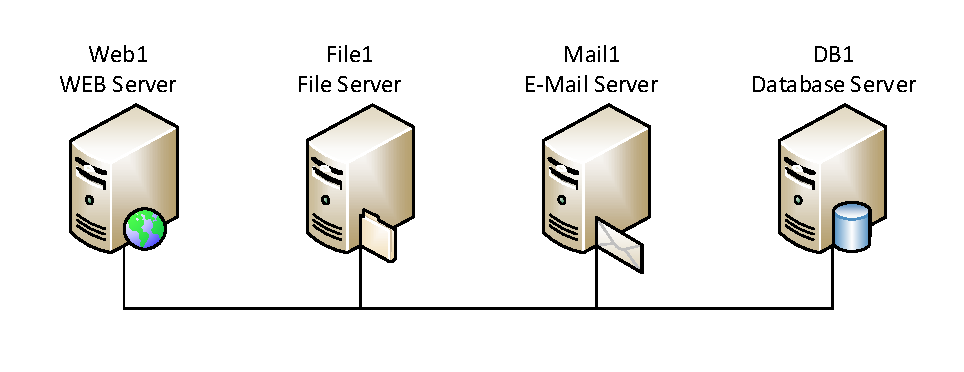
\includegraphics[scale=0.6]{img/servicegroup_layout}
    \caption{Tjenester for servicegroup-objektet  ERP\_WEBAPP}
    \label{servicegroup_layout}
\end{figure}


Konfigurasjonen for dette er vist under. Direktivet “Members” setter medemene i gruppen der hvert service-objekt er “host\_name,service\_description”.

\begin{lstlisting}
define servicegroup {
	servicegroup_name ERP_WEBAPP
	alias Web App for ERP
	members Web1,Check HTTP, File1,Check SMB, Mail1,Check Exchange, DB1,Check MySQL
}
\end{lstlisting}


Her kjøres service-sjekker mot alle tjenestene. Service-objektene grupperes i en servicegroup. 
Dette gjør at vi får et oversiktsbilde over applikasjonen i Icingas web-grensesnitt som vist i Figur \ref{servicegroup_web}. Slik blir det enklere for servicedesk å kunne gå inn for å se hva som er feil med “Web app for ERP” om brukere rapporterer om feil på applikasjonen.

\begin{figure}
    \centering
    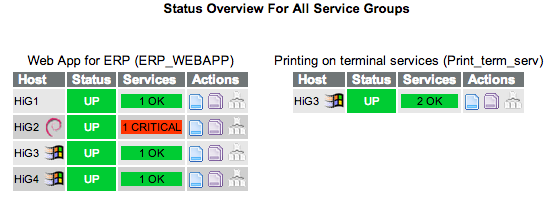
\includegraphics[scale=0.6]{img/servicegroup_web}
    \caption{ Oversikt over servicegroup-objekt og status i webgrensesnittet}
    \label{servicegroup_web}
\end{figure}

Det vil det også være naturlig å sette opp servicedependency-er mellom ERP Web1 og sjekkene for webserveren, filserveren, mailserveren og databaseserveren.

\section{Infrastruktur}
Infrastruktur består av de grunnleggende enhetene de andre serverne er avhengig av. I dette prosjektet er det definert til: switcher, routere, brannmurer, UPS, virtualiseringsteknologi og serverrommiljø.

Infrastrukturovervåkning er essensielt for å kunne levere IT-Tjenester. Det er viktig at design av overvåkningen fører til at man raskt og effektivt skal kunne oppdage og presentere feil som oppstår. For å få til dette i Icinga benyttes “parent” /ref{parents}. De aller fleste enheter i infrastrukturen (untatt servermiljø) vil være parent for andre enheter. Dette reflekteres i et statuskart i icinga, som vist i Figur \ref{statusmap}.

\begin{figure}
    \centering
    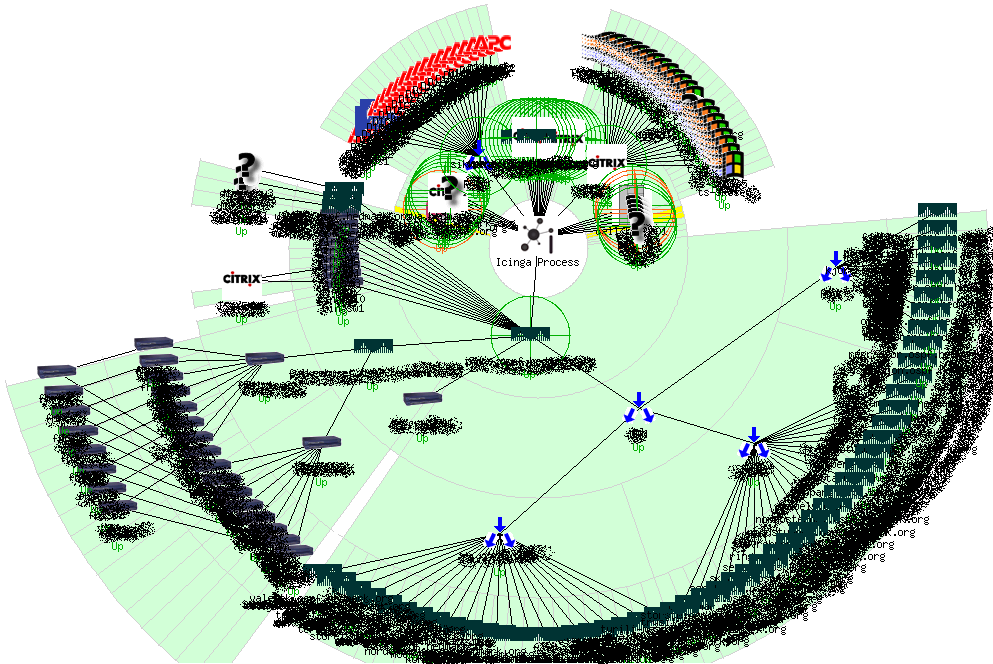
\includegraphics[scale=0.6]{img/statusmap}
    \caption{Kart som viser parent og host-relasjoner}
    \label{statusmap}
\end{figure}


\subsection{Switcher}
Switcher er nettverksutstyr som jobber på lag 2 i OSI modellen. IKT-avdelingen benytter switcher med lag 3 funksjonalitet. Lag 3 funksjonalitet vil si at switchen kan kommunisere over IP. Alle switchene IKT-avdelingen benytter støtter SNMP-protokollen, som brukes til overvåkingen.

På switchene overvåkes forskjellige sensorer avhengig av hva de inneholder. Alle switcher har for eksempel ikke vifter.

Det er laget et generisk oppsett som overvåker temperatur, PSU og viftestatus. Hvilken OiD denne informasjonen ligger under varierer fra leverandøren til leverandør. Mange produsenter benytter også samme OiD. 

Dersom en vifte eller PSU raporteres som defekt vil det raporteres som en CRITICAL-status i Icinga. For temperatur er grenseverdiene satt til xx for WARNING og xx for CRITICAL.

Switchene IKT-Avdelingen bruker er forskjellige modeller fra leverandørne Cisco, Dell og HP. Disse overvåkes med plugin-ene "check\_nwc\_health" \cite{nwchealth} for Cisco og HP og check\_snmp\_powerconnect for Dell \cite{checkpowerconnect}.

\subsection{Routere og brannmurer}
IKT-avdelinger benytter Cisco ASA og Cisco PIX routere mellom forskjellige subnettverk. I tillegg utfører de gjerne oppgaver som pakkefiltrering, NAT og IPsec-tunneler.
% TODO: Sjekk at dette er riktig mot docs
\subsubsection{Ressurser}

Som for switcher \ref{switch} brukes check\_nwc\_health til å se at sensorer er OK. I tillegg
sjekkes CPU-bruk og minneforbruk gjennom samme plugin. 

For CPU-bruk sjekkes gjennomsnittet over 5 minutter. Grenseverdier er satt til 80 \% på WARNING og 90 \% på CRITICAL, i henhold til det cisco anbefaler \cite{ciscounifiedcommunication}. Høy CPU-bruk kan føre til dårligere ytelse, høy rate av buffer-feil og generelle feil med responsivitet \cite{ciscocpurouters}

I følge Cisco kan høytminneforbruk under vanlig operasjon indikere at brannmuren er under angrep. \cite{ciscomem}. Dersom en router bruker opp tilgjengelig minne kan det føre til at routeren slutter å svare på kommandoer, telnet-tilkoblinger eller henger \cite{ciscomemproblem} . Cisco anbefaler en grenseverdi på 15 \% ledig minne \cite{ciscounifiedcommunication}. Grenseverdier for minne er derfor satt til 20 \% for WARNING og 15 \% for CRITICAL.

\subsubsection{Failover}

Cisco router / Brannmurer har en viktig funksjon som kalles failover. Denne fungerer slik at to like enheter settes opp, der en blir satt som “primary” og den andre som “secondary”, slik at denne kan overta for “primary” om det skulle bli nødvendig. Disse kobles sammen med en seriellkabel. Figur \ref{ciscoasafailover} viser hvordan et Cisco-failover er satt opp. 

\begin{figure}
    \centering
    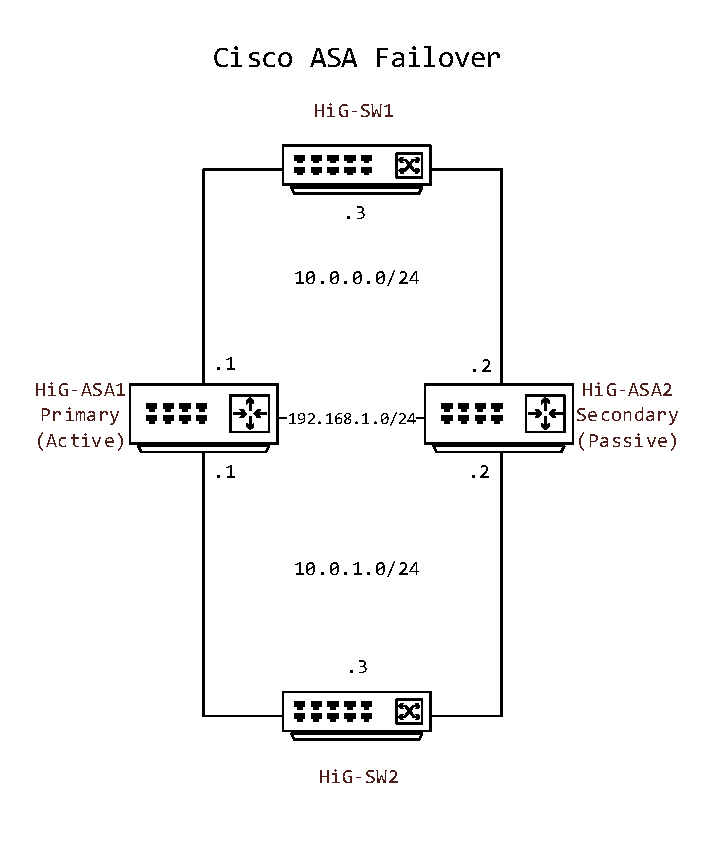
\includegraphics[scale=0.6]{img/asafailover}
    \caption{Oppsett for Cisco-failover funksjonalitet}
    \label{ciscoasafailover}
\end{figure}


Dersom primary går ned vil secondary ta over nødvendige ruter, brannmurregler og konfigurasjon. Secondary vil dermed overta IP- og MAC-adressen til primary. Primary vil bli satt som passiv (trenger ikke nødvendigvis å ha en passiv IP adresse, fordi IP kommunikasjon går kun gjennom det aktive interfacet) helt til en manuelt endrer dette tilbake i konfigurasjonen. \cite{ciscofailover}. 

Sjekkene som settes opp for å verifisere at failover funksjonaliteten fungerer som den skal, og at det ikke har intruffet feil er:
\begin{itemize}
\item Hvis primary er satt som aktivt og secondary er passiv returneres OK.
\item Om primary er satt som passiv returneres WARNING. 
\item Om secondary er satt som aktiv returneres WARNING.
\item Hvis primary eller secondary får en error returneres CRITICAL
\item Hvis failover ikke er konfigurert returneres UNKNOWN. 
\end{itemize}

Til dette benyttes pluginen “check\_cisco\_firewall” \cite{checkciscofirewall}.

Hvis brannmurene deler management IP på primary og secondary, er det ingen mulighet for å hente ut informasjon fra den passive brannmuren. Da sjekkes failover status bare for primary. I et ideelt miljø burde både passiv og aktiv ha hver sin IP adresse, slik at fysiske feil kan avdekkes på den passive brannmuren.

Begge brannmurene legges i en hostgroup som er lagt på service-objektet for “cisco\_health” slik at lokale ressurser sjekkes på samme måte som switcher. Brannmurene legges også inn i en hostgroup som heter Cisco-failover som benyttes i service-objektet for failover.

\subsubsection{VPN}

For brannmurer som har VPN-tjeneste sjekkes antall oppkoblede bruker opp mot det antallet brannmuren er lisensiert for. Begge disse verdiene finnes som SNMP OID-er definert i CISCO-FIREWALL-MIB. Det fantes allerede en plugin som sjekker antall tilkoblede brukere \cite{checkciscovpn}. Denne ble endret til å også hente ut det maksimale antallet og sammeligne brukt kapasitet i prosent mot grenseverdier som kommer inn som argumenter.

\subsubsection{Båndbredde}

For å overvåke båndbreddebruk ut av og inn på en port Cisco ASA og PIX finnes to muligheter:

\subsubsection*{Netflow}

Funksjonen Netflow \cite{ciscoiosnetflow} fungerer ved at enheten samler inn informasjon om og statistikk over alle pakker som går ut og inn av portene. Dette krevet at Netflow konfigureres på alle routerne og det vil også ta opp ekstra minne og CPU \cite{cisconetflowperf}. Derfor ble det avgjort å ikke benytte Netflow.

\subsubsection*{Telle pakker}

Både Cisco Pix og ASA har tellere for antall byte som går ut og inn på en nettverksport. For å kalkulere båndbredde bruk over et intervall kan en hente ut disse, vente en gitt periode og hente ut nye verdier. Da vil bruken være ((målepunkt2 - målepunkt1)*8) / antall sekunder.

Mange plugins benytter seg dette ved å lese ut “ifInOctets” og “ifOutOctets” over SNMP. Det er også disse som er benyttet i Ciscos notat “How to Calculate Bandwidth Using SNMP” \cite{ciscobandwidth}. 

En stor ulempe med å benytte disse er at de er 32 bit, og vil dermed nullstilles kjapt ved høye hastigheter. For 1000Mbps vil tiden det vil ta til telleren går rundt være ((2\^32)-1) / ((10\^9)/8) = ca. 34 sekunder. Se Tabell /ref 
\begin{table}
\begin{center}
\begin{tabular}{ | l | p{7cm} |} 
        \textbf{Hastighet} & \textbf{Tid}
	\\ \hline
        10 Mbps & 57 minutter og 15.97 sekunder \\ \hline  
        100 Mbps & 5 minutter og 43.60 sekunder \\ \hline
	1000 Mbps & 34.36 sekunder \\ 
	\hline
\end{tabular}
\label{kalkulering_teller}
\end{center}
\end{table}
Det er derfor anbefalt å bruke 64-bit-variablene ifHCOutOctets og ifHCInOctets i stedet \cite{ciscosnmpcounters}.

Pluginen det er tatt utgangspunkt i for å hente ut båndbreddebruk heter check\_iftraffic64 \cite{checkciscoif}. Denne er noe omskrevet for å kunne sende inn absolutte verdier som grenseverdier for varsling. I generic-firewall er det satt opp to egendefinerte variabler “WANWARN” og “WANCRIT”, som setter standard grenseverdier for alle brannmurer. For brannmurer der det er normalt med høyere båndbreddebruk er disse variablene overstyrt i konfigurasjonen for host-objektet.

\subsection{VMware og Citrix Xen}

Ved IKT-avdelingen er det både et Citrix Xen-miljø og et VMware-miljø. Disse består av servere som kjører hypervisorene ESX 5.1 og Xen 6. Begge er av typen 1 (direkte på hardware) og står for administering av virtuelle maskiner, som er operativsystemer med applikasjoner. Hypervisoren introduserer altså  et nytt lag mellom hardware og applikasjonene brukeren benytter. Host-ene har ansvaret for at de virtuelle maskinene får tilstrekkelig med ressurser for å kunne kjøre applikasjoner installert. 

For overvåkning av virtuelle maskiner brukes NRPE, det overvåkes da som en “egen” server. Overvåkning av servere som kjører hypervisor-ene vil bestå av å sjekke om ressurser strekker til etterspørselen fra de virtuelle maskinene. En eller flere virtuelle maskiner kan kreve mer ressurser enn en server har fysisk. Dette stjeler både CPU-tid, minne og I/O for å håndtere, noe som vil gå utover gjeste-operativsystem og applikasjoners responstid. Videre vil overvåkning av hvor mye ressurser som brukes gi muligheten for å kalkulere når eventuelle skaleringstiltak må innføres. /ref http://pubs.vmware.com/vsphere-51/topic/com.vmware.ICbase/PDF/vsphere-esxi-vcenter-server-51-monitoring-performance-guide.pdf

\subsubsection{VMware}

Pluginen “check\_vmware\_api.pl”, som er utviklet av et open source firmaet op5 /ref http://www.op5.com/, er brukt for å hente ut informasjonen fra VMware vCenter. Denne pluginen bruker et SDK-bibliotek i Perl /ref http://www.vmware.com/support/developer/viperltoolkit/ for å utføre API-kall til vCenter. Autentisering skjer ved å sende med brukernavn og passord for en brukerkonto som opprettet i vCenter-serveren med read-rettigheter. For å utveksle informasjon blir SOAP-protokollen benyttet/ref http://en.wikipedia.org/wiki/SOAP via HTTPS. 

http://docwiki.cisco.com/wiki/Troubleshooting\_and\_Performance\_Monitoring\_Virtualized\_Environments

\begin{enumerate}
	\item hvert 5 minutt over en dag 
	\item hvert 30 minutt i en uke
	\item hver 2. time i en måned
	\item en dag over ett år
\end{enumerate}

Pluginen i CLI

./check\_vmware\_api.pl -D <vCenter ip> -u <brukernavn> -p <passord> | -H <host\_navn> -N <vm\_navn> -C <cluster\_navn>  -l <hovedkommando> -s <subkommando> -i <interval> -T <timeshift>

For å overvåke flere parametere kan en legge til kode i pluginen så lenge ønskede parametere er tilgjengelig via API-et. Navnet på funksjoner følger standarden:

<host eller vm eller cluster>\_<hovedkommando>\_info 

Så for eksempel for å legge til en ny CPU-parameter finner en “host\_cpu\_info” funksjonen og legger til en elseif på subkommandoen som brukes for å referere til et gitt parameter i VMware API-et. En kan følge oppsettet på de pluginen som allerede er definert. Dett krever noe kunnskaper om språket Perl.

For alle parametere som blir hentet ut blir tilleggsoppsjonene -i 300 og -T 300 sendt med.
Som nevnt over lagres data i ulike intervall, og opsjonen “-i 300” vil si at det hentes ut data med intervall-ID 300 og vi får da gjennomsnittet for 5 minutter med datapunkt for hvert 20 sekund (standard innhenting i vCenter). Opsjonen “-T” er timsehift i sekunder, som vil si at det returneres data i fra tiden sjekken blir kjørt og 300 sekunder tilbake i tid. 

Etter analyse av output fra pluginen ble det observert at dette var innstillingene som ga oss data om det siste 5 minutters-intervallet. Dette var ønskelig fordi pluginen varsler mot det siste intervallet, så de andre intervallene var overflødige. Andre opsjoner som ble testet var bare “-i 300”, men her kom det 288 resultater tilbake. Dette er antall datapunkt som blir generert i 5 minutters intervallet for en dag. /ref http://pubs.vmware.com/vsphere-51/index.jsp?topic=2Fcom.vmware.wssdk.pg.doc2FPG\_Performance.18.6.html

To counters har blitt tatt ut for overvåkning , og vil være eksempel på hvordan en setter opp sjekker. Disse kan brukes som referanse for utvidelse av overvåkningen av VMware. 

 Parametere som nå overvåkes: : 
/citehttp://docwiki.cisco.com/wiki/Troubleshooting\_and\_Performance\_Monitoring\_Virtualized\_Environments
/citehttp://pubs.vmware.com/vsphere-51/topic/com.vmware.ICbase/PDF/vsphere-esxi-vcenter-server-51-monitoring-performance-guide.pdf

\subsubsection*{CPU}

/cite http://www.vmware.com/support/developer/vc-sdk/visdk400pubs/ReferenceGuide/cpu\_counters.html


Counter usage.average (\%) over siste 5 minutt -  warning: 75 critcal: 90 

``Actively used CPU of the host, as a percentage of the total available CPU. Active CPU is approximately equal to the ratio of the used CPU to the available CPU. available CPU = \# of physical CPUs x clock rate''

Grenseverdier her er satt til samme nivå som tilsvarende alarm i vCenter, og gir indikasjon på at det kan være en eller flere virtuelle maskiner som krever for mye CPU i forhold til hva hosten har tilgjengelig. Det kan også være et for stort antall virtuelle maskiner på hosten. 

\subsubsection*{Minne}

Counters 

 usage.average (\%) warning: 80 critical: 90

“Percentage of available machine memory: consumed ÷ machine-memory-size”

Grenseverdier her er satt til samme nivå som vCenter, og vil gi indikasjon på om virtuelle maskiner krever mer minne enn hosten har tilgjengelig. Når det er igjen 6\% minne (free) vil hosten iverksetter enten ballooning og eventuelt swapping. Disse to reallokeringsteknikken krever CPU kraft og er en indikasjon på at minneforbruket er for høyt

\subsubsection{Xen}

For overvåkning av Xen-miljøet er det foreløpig en plugin etter det vi fant som gir muligheten til å hente ut informasjon fra hosts og virtuelle maskiner. Pluginen check\_xen\_api.pl, utnytter kall via url mot en RRD-database hvor xapi lagrer data /cite http://wiki.xen.org/wiki/XAPI\_RRDs. 
Antall parametere som er tilgjengelige er ikke like stort som for eksempel VMware. I/O data er foreløpig ikke tilgjengelig, og relevant data er CPU og minnebruk.

RRD-databasen lagrer data i følgende intervall:
\begin{enumerate}
	\item Hvert 5 sekund i en 10 minutters periode
	\item Hvert minutt i en 2 timers periode
	\item Hver time i en ukers periode
	\item Hver dag for ett år
\end{enumerate}

For hvert 5 sekund blir aktuelle datapunkt lagret, og for de tre andre en gjennomsnitts funksjon kjørt og gjennomsnittet fra den aktuelle tidsperioden blir lagret 

Parametere som er valgt for å overvåke Xen hosts:

CPU bruk i prosent - warning: 80 critical: 90 

Total bruk for alle kjerner / antall kjerner

Minne bruk (MB og \%, varsler på \%) - warning: 80 critical: 90

Totalt allokert minne - ledig minne 

Et problem ble støtt på under implementeringen av check\_xenplugin.api som fikk stor innvirkning på returnert resultat fra RRD-databasen. Etter å ha lest gjennom koden til selve pluginen og “biblioteket” XenAPI som også er skrevet av op5, ble det oppdaget at denne pluginen bruker siste datapunkt fra intervall nr.1 nevnt over. Resultatet vil da bare være ett datapunkt. Dette er vanskelig å sette varsel på, da en spike kan skje når gitt sjekk kjører. Her ble det avgjort å legge til en ny opsjon for å angi over hvor lang tidsperiode en skal hente ut data. Returnert resultat fra gitt tidsperiode blir gått gjennom og en gjennomsnittsverdi av dette returnert. Dette er foreløpig bare implementert for CPU- og minnebruk for en host.

\subsection{Trådløse kontrollere}

De trådløse kontrollerne som benyttes av IKT-avdelingen mangler støtter for SNMP-get for informasjon som hentes ut fra switcher og brannmurer som  CPU- og minnebruk. Dette vil i følge produsenten komme i en senere firmware-oppdatering.
Noe av dette kan løses ved å bruke SNMP-traps i stedet og definere verdier for når disse skal sendes ut direkte på kontrollerne. Her ble traps som omhandler kontrollerne og var relevante for IKT-avdelingen satt opp:

\begin{itemize}
	\item Hardware feil med kontrolleren
	\item Ressursmangel på kontrolleren
	\item Rogue AP - et udefinert aksesspunkt er oppdaget av de andre aksesspunktene.
	\item Failover til annen kontroller
	\item Feil med kontakt mot Radius
	\item Lisens utløpt
\end{itemize}

For å få til dette trengs et mellomledd som kan motta SNMP-traps på Icinga-serveren, tolke trap-meldingene og sende informasjonen videre til Icinga. 

For å lytte etter SNMP-traps benyttes SNMPtrapd (http://www.net-snmp.org/docs/man/snmptrapd.html). Her mottas alle traps som sendes med riktig community. Disse sendes så videre til snmptt (SNMP Trap Translator - http://snmptt.sourceforge.net/). Her har defineres de traps-ene en er ute etter, informasjon om OID-ene og kommandoen som skal kjøres når denne mottas. I Figur \ref{snmptrap} illustreres hvordan en trap blir prosessert. 

\begin{figure}
    \centering
    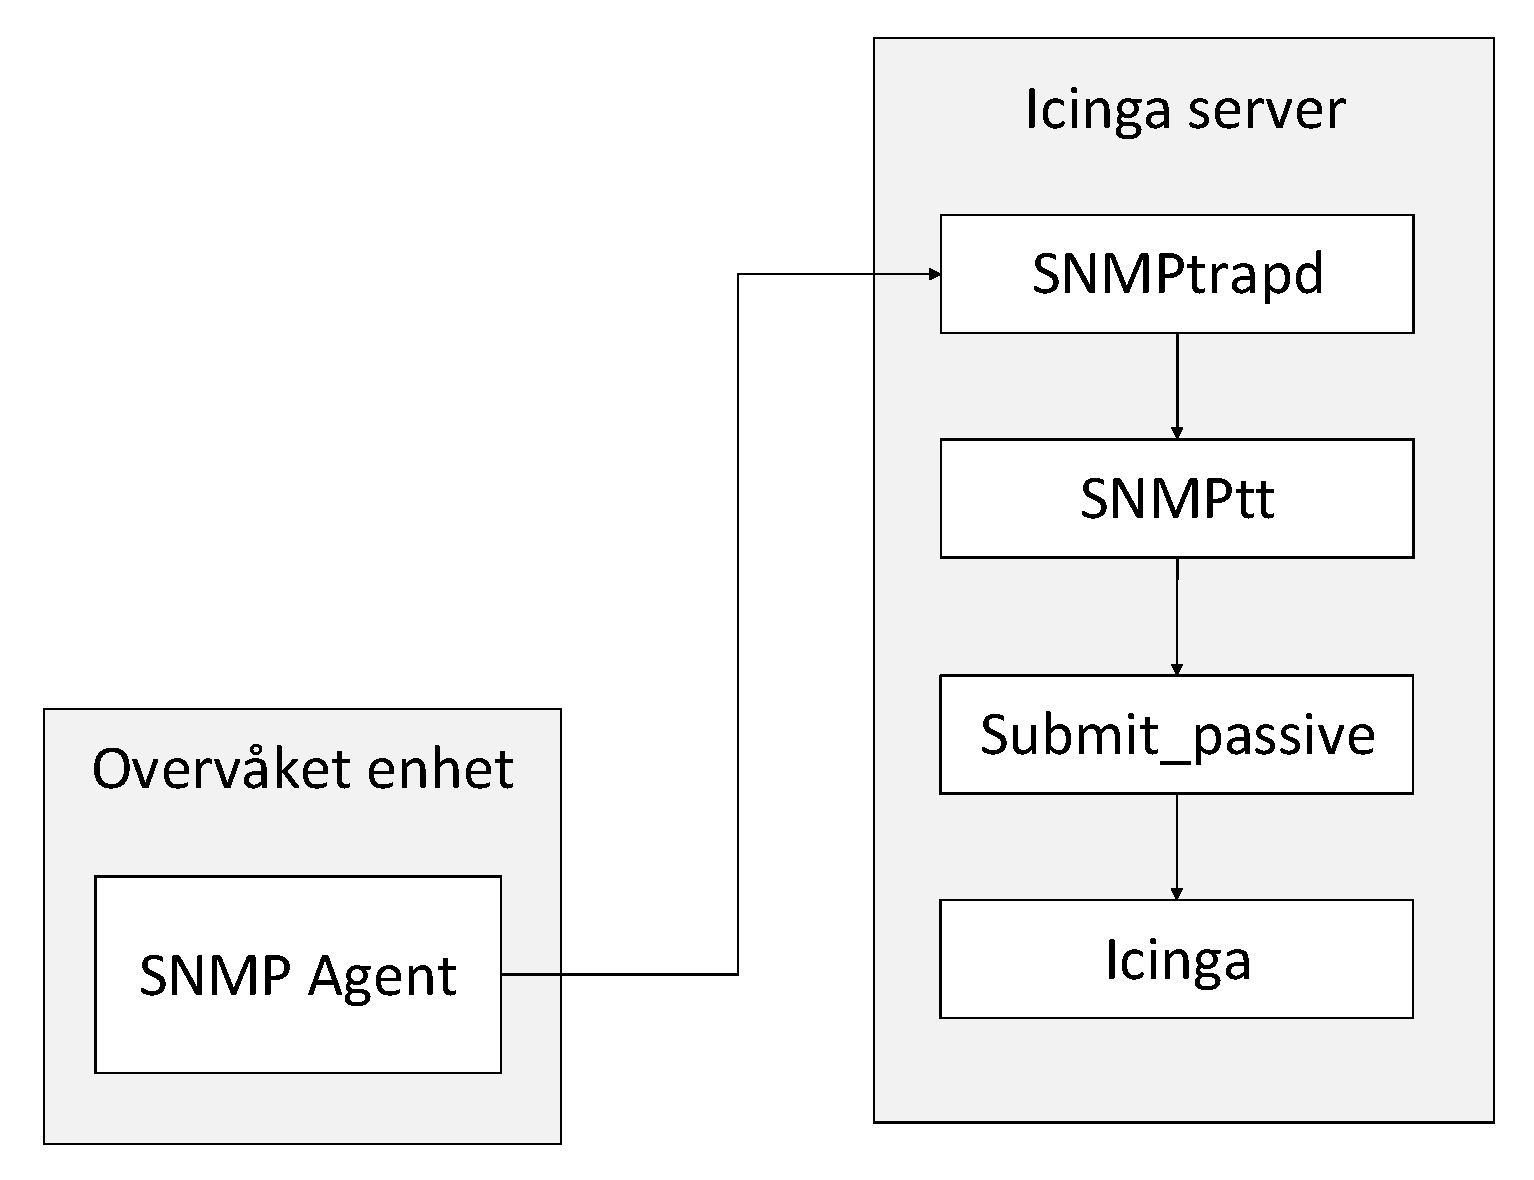
\includegraphics[scale=0.6]{img/SNMPtrap}
    \caption{Informasjonsflyt ved en trap}
    \label{snmptrap}
\end{figure}

SNMPtt trenger konfigurasjon for alle OID-ene som skal prosesseres. Disse kan opprettes med snmpttconvertmib ut i fra en MIB-fil slik:

\begin{lstlisting}
root@icinga1:/usr/share/mibs/netsnmp# snmpttconvertmib --in=MERU-WLAN-MIB.my --out=meru.conf --exec='/usr/lib/nagios/plugins/libexec/submit_check_result "$aA meru_$N 2 $D"
\end{lstlisting}

Eksempel på en OID som blir generert i filen meru.conf:

\begin{lstlisting}
EVENT mwlRogueApDetected .1.3.6.1.4.1.15983.3.1.3.13 "Status Events" Normal
FORMAT $*
EXEC /usr/lib/nagios/plugins/libexec/submit_check_result $aA meru_$N 2 "$D"
SDESC
A rogue AP is detected. The AP id, mac address, and other information are described in mwlTraContent.
EDESC
\end{lstlisting}

Her benyttes variabler i snmptt (cite http://snmptt.sourceforge.net/docs/snmptt.shtml\#Variable-substitutions):
\begin{itemize}
	\item IP-adressen til snmp agenten, altså kontrollereren
	\item Navnet på trap-en
	\item Beskrivelse på trap fra konfigurasjonfila.
\end{itemize}

SNMPtt vil så kjøre kommandoen definerte under “EXEC” for OID-en, som for dette tilfellet er å sende informasjonen videre til scriptet “submit\_check\_result”. Dette tar fire argumenter:

\begin{itemize}
	\item IP-adresse eller hostname 
	\item Service description
	\item Returkode som setter status på tjenesten (0-3)
	\item Plugin-output
\end{itemize}

Service description for alle meru traps som sendes inn vil da være “meru\_” + navnet på trap-en. Som plugin-output er det lagt inn beskrivelse av trap-en, da denne som regel er noe mindre kryptisk en navnet.

Scriptet vil så skrive dette sammen med et timestamp til icinga.cmd som Icinga sjekker periodisk etter resultat av passive sjekker.

En ting å merke seg her er at en ikke vil få informasjon når tjenesten er OK igjen, og må sette tjenestene til OK manuelt i Icingas webgrensesnitt.

\subsection{Serverrommiljø}

For å overvåke temperatur og luftfuktighet på serverrommet ble det kjøpt inn en APC NetBotz 200 \ref{https://www.apc.com/products/family/index.cfm?id=346} med fire eksterne sensorer. Disse ble plassert slik at det er to sensorer på hver side av rack-raden. En vil dermed kunne se temperaturforskjellen mellom forsiden av serverne, ved luftinntak og baksiden, der varmluft går ut.

Hver sensor måler både temperatur og luftfuktighet. For luftfuktighet støttes bare relativ luftfuktighet.

\subsubsection{Luftfuktighet}

Relativ luftfuktighet er definert som “forholdet mellom partielltrykket til vanndamp, i en gassblanding av luft og vann, og vanndampens metningstrykk ved en viss temperatur. som gir oss prosentandelen av vann i luften. (cite http://no.wikipedia.org/wiki/Luftfuktighet). 

Det er også mange enheter som overvåker duggpunkt, som vil si temperaturen en viss mengde luft må avkjøles til for at vanndamp skal kondensere. Ved en økning i relativ luftfuktighet vil duggpunktet nærme seg luftemperaturen. Ved 100\% relativ luftfuktighet vil temperaturen og duggpunktet være like. 

I “Sun Microsystems Data Center Site Planning Guide” anbefales en luftfuktighet på 45 \% - 50 \%. Det meste av datautstyr kan fungere innenfor et bredere intervall enn det, typisk 20 \% - 80 \%. Men de anbefalte verdiene er satt for at det skal være et buffer dersom en har klimaanlegg som kontrollerer luftfuktighet, og det slutter å fungere. /cite http://docs.oracle.com/cd/E19065-01/servers.e25k/805-5863-13/ch3.html\#98939 Andre, som “American Society of Heating, Refrigerating and Air-Conditioning Engineers” (ASHRAE) anbefaler at den relative luftfuktigheten ikke bør overstige 60 \%, mens den nedre gresen er basert på duggpunkt og satt til 5.5°C, der den relative luftfuktigheten vil variere mellom 25 \% og 45 \% /cite http://tc99.ashraetcs.org/documents/ASHRAE\_Extended\_Environmental\_Envelope\_Final\_Aug\_1\_2008.pdf. Disse verdiene er også anbefalt av Cisco cite http://www.cisco.com/en/US/solutions/collateral/ns340/ns517/ns224/ns944/white\_paper\_c11-680202.pdf, og omtalt som vidt akseptert. 

For høy luftfuktighet kan føre til kondens, som igjen kan føre til korrosjon på komponenter. Ved lavere luftfuktighet øker faren for utladninger av statisk elektrisitet (kritisk ved 30 \%), som kan føre til utladninger med ekstremt høye spenningsverdier, som kan ødelegge komponenter.

\subsubsection{Temperatur}

Det er mye uenighet rundt anbefalte verdier for temperatur i serverrom. I et studie utført ved University of Toronto /cite http://dl.acm.org/citation.cfm?id=2254778, ble det samlet inn data fra tre forskjellige organisasjoners datasentre, deriblant Googles. I studiet ble det konkludert med at faren for hardware-feil ved høyere temperatur øker mindre enn det som har vært vanlig å basere seg på. For DRAM-feil og ``node outages'' fant de ingen korrelasjon til temperaturøkning for intervallet i testen (15°C - 60°C). I dette studiet ble det ikke målt eller tatt hensyn til luftfuktighet. 

ASHRAE anbefaler en inntakstemperatur 18°C - 27°C, mens Sun anbefaling er 20°C - 23°C. Sun bregrunner sin anbefaling med at det er lettere å opprettholde trygge verdier for relativ luftfuktighet. ASHRAE viser også til studier som viser at det totale strømforbruket kan gå opp ved høyere temperaturer fordi enheter øker frekvensen på egne vifter. http://ieeexplore.ieee.org/xpl/login.jsp?tp=\&arnumber=4544393\&url=http\%3A\%2F\%2Fieeexplore.ieee.org\%2Fxpls\%2Fabs\_all.jsp\%3Farnumber\%3D4544393

\subsubsection{Plugin for overvåkning av temperatur og luftfuktighet i Icinga}

Det fantes allerede en plugin for å sjekke sensorverdiene på APC NetBotz (http://exchange.nagios.org/directory/Plugins/Hardware/UPS/APC/check\_netbotz/details). Men denne sammenlignet verdiene med grenseverdier satt i konfigurasjonen på enheten. Det var ønskelig å samle mest mulig av konfigurasjon på Icinga-serveren, derfor ble pluginen omskrevet til å kunne ta inn øvre og nedre grenseverdier som argumenter.

\subsubsection{UPS (Uninterruptible Power Supply)}

UPS, på norsk ofte kalt avbruddsfri strømforsyning blir benyttet til å opprettholde strøm til alle enheter på IKT-avdelingens serverrom, dersom strømnettet skulle falle ut og filtrere den strømen slik at utstyr ikke vil bli skadet om spenningen skulle spike.

Ved IKT-avdelingen benyttes UPS-er av fabrikatene APC og HP.

For APC overvåkes:
\begin{itemize}
 	\item Battery capacity - igjen av charge
	\item load
	\item voltage in/out
	\item internal temp
\end{itemize}

For HP overvåkes:
\begin{itemize}
	\item voltage in/out
	\item Battery current
	\item battery capacity
\end{itemize}

For både HP og APC overvåkes alle parametere direkte over SNMP med pluginen “check\_snmp” fra nagios-plugins. Her er OID-ene definert direkte i service-objektene.
